% Copyright (c) 2026 Islam Ibrahim. All rights reserved.

\documentclass[tikz,border=10pt]{standalone}
\usepackage[T1]{fontenc}
\usepackage{lmodern}
\usepackage{amsmath,amssymb}
\usepackage{tikz}
\usetikzlibrary{arrows.meta,decorations.pathreplacing,positioning}

\begin{document}
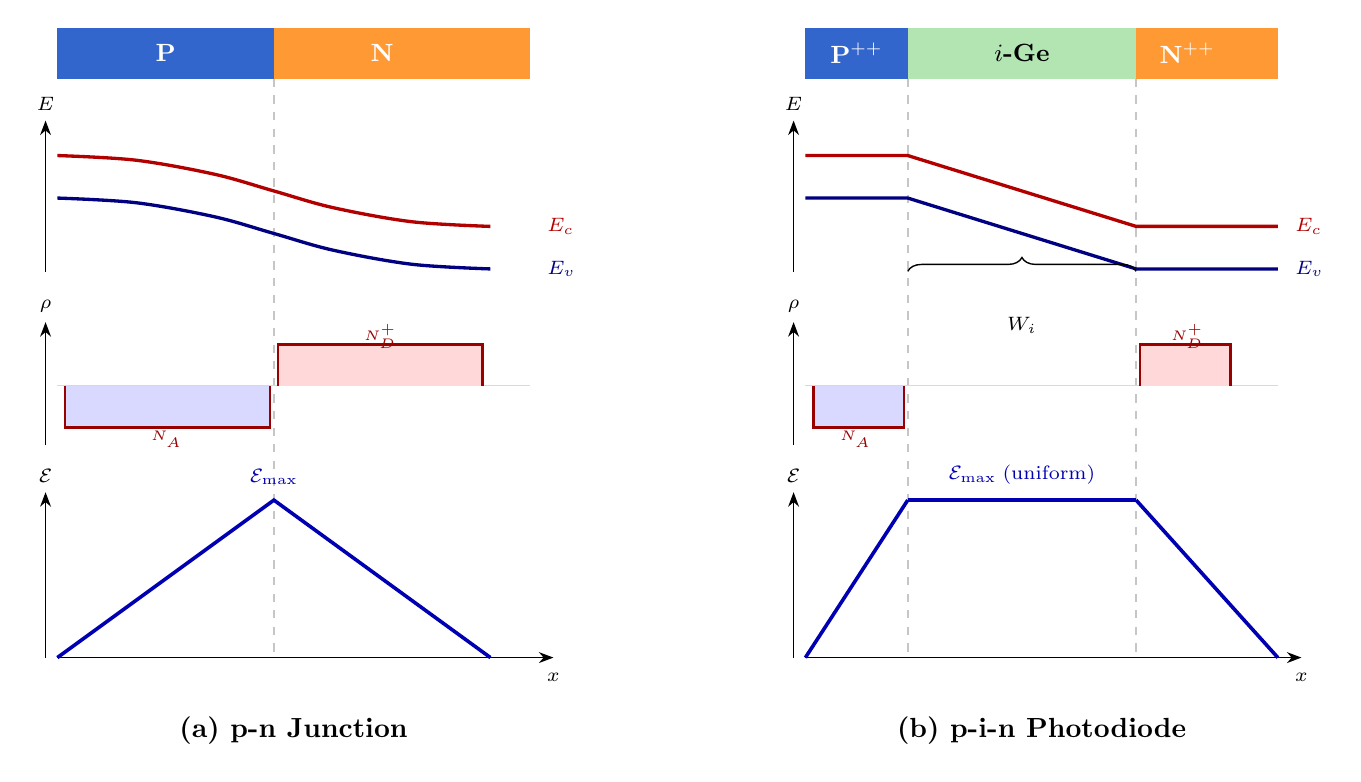
\begin{tikzpicture}[font=\footnotesize\rmfamily, >=Stealth]

%% Dimensions
\def\PW{6.0}
\def\EFh{2.0}
\def\CDh{1.5}
\def\BDh{1.8}
\def\subgap{0.70}
\def\stripH{0.65}
\def\stripGap{0.65}
\def\hgap{3.5}
\def\Eg{0.30}

%% Vertical positions
\pgfmathsetmacro{\EFbot}{0}
\pgfmathsetmacro{\EFtop}{\EFh}
\pgfmathsetmacro{\CDbot}{\EFtop+\subgap}
\pgfmathsetmacro{\CDtop}{\CDbot+\CDh}
\pgfmathsetmacro{\BDbot}{\CDtop+\subgap}
\pgfmathsetmacro{\BDtop}{\BDbot+\BDh}
\pgfmathsetmacro{\stripBot}{\BDtop+\stripGap}
\pgfmathsetmacro{\stripTop}{\stripBot+\stripH}

%% Colors
\definecolor{pcolor}{RGB}{51,102,204}
\definecolor{icolor}{RGB}{178,229,178}
\definecolor{ncolor}{RGB}{255,153,51}
\colorlet{efieldCol}{blue!70!black}
\colorlet{ecCol}{red!70!black}
\colorlet{evCol}{blue!50!black}
\colorlet{rhoCol}{red!60!black}

%% ============================================================
%% Column (a) — p-n Junction
%% ============================================================
\begin{scope}[shift={(0,0)}]
  % Region strip
  \fill[pcolor] (0,\stripBot) rectangle (2.75,\stripTop);
  \node[font=\small\bfseries,white] at (1.375,\stripBot+\stripH/2) {P};
  \fill[ncolor] (2.75,\stripBot) rectangle (\PW,\stripTop);
  \node[font=\small\bfseries,white] at (4.125,\stripBot+\stripH/2) {N};

  \draw[gray!45,dashed,line width=0.6pt] (2.75,\stripBot) -- (2.75,\EFbot);

  % Band diagram
  \draw[->,line width=0.5pt] (-0.15,\BDbot) -- (-0.15,\BDtop+0.12)
    node[at end,above=0pt,font=\scriptsize] {$E$};

  \pgfmathsetmacro{\ecAa}{\BDbot+0.82*\BDh}
  \pgfmathsetmacro{\ecAb}{\BDbot+0.32*\BDh}
  \pgfmathsetmacro{\totalDrop}{\ecAa-\ecAb}

  \draw[ecCol,line width=1.2pt] plot[smooth,tension=0.55] coordinates {
    (0.0,\ecAa) (1.0,{  \ecAa-\totalDrop*0.066})
    (2.0,{\ecAa-\totalDrop*0.265}) (2.75,{\ecAa-\totalDrop*0.500})
    (3.5,{\ecAa-\totalDrop*0.735}) (4.5,{\ecAa-\totalDrop*0.934})
    (5.5,\ecAb)
  };
  \node[ecCol,font=\scriptsize,right] at (\PW+0.1,\ecAb) {$E_c$};

  \pgfmathsetmacro{\EgOff}{\Eg*\BDh}
  \draw[evCol,line width=1.2pt] plot[smooth,tension=0.55] coordinates {
    (0.0,{\ecAa-\EgOff}) (1.0,{\ecAa-\EgOff-\totalDrop*0.066})
    (2.0,{\ecAa-\EgOff-\totalDrop*0.265}) (2.75,{\ecAa-\EgOff-\totalDrop*0.500})
    (3.5,{\ecAa-\EgOff-\totalDrop*0.735}) (4.5,{\ecAa-\EgOff-\totalDrop*0.934})
    (5.5,{\ecAb-\EgOff})
  };
  \node[evCol,font=\scriptsize,right] at (\PW+0.1,{\ecAb-\EgOff}) {$E_v$};

  % Charge density
  \draw[->,line width=0.5pt] (-0.15,\CDbot) -- (-0.15,\CDtop+0.06)
    node[at end,above=0pt,font=\scriptsize] {$\rho$};
  \pgfmathsetmacro{\CDzero}{\CDbot+\CDh/2}
  \draw[gray!30,line width=0.4pt] (0,\CDzero) -- (\PW,\CDzero);

  \fill[blue!15] (0.1,\CDzero) rectangle (2.70,{\CDbot+0.15*\CDh});
  \draw[rhoCol,line width=0.9pt] (0.1,\CDzero)--(0.1,{\CDbot+0.15*\CDh})
    --(2.70,{\CDbot+0.15*\CDh})--(2.70,\CDzero);
  \node[rhoCol,font=\tiny] at (1.4,{\CDbot+0.08*\CDh}) {$N_A^-$};

  \fill[red!15] (2.80,\CDzero) rectangle (5.4,{\CDbot+0.85*\CDh});
  \draw[rhoCol,line width=0.9pt] (2.80,\CDzero)--(2.80,{\CDbot+0.85*\CDh})
    --(5.4,{\CDbot+0.85*\CDh})--(5.4,\CDzero);
  \node[rhoCol,font=\tiny] at (4.1,{\CDbot+0.92*\CDh}) {$N_D^+$};

  % Electric field (triangle)
  \draw[->,line width=0.5pt] (-0.15,\EFbot) -- (-0.15,\EFtop+0.10)
    node[at end,above=0pt,font=\scriptsize] {$\mathcal{E}$};
  \draw[->,line width=0.5pt] (0,\EFbot) -- (\PW+0.3,\EFbot)
    node[at end,below=2pt,font=\scriptsize] {$x$};

  \draw[efieldCol,line width=1.3pt] (0,\EFbot)--(2.75,\EFtop)--(5.5,\EFbot);

  \node[efieldCol,font=\scriptsize,above=2pt] at (2.75,\EFtop) {$\mathcal{E}_\mathrm{max}$};

  \node[font=\normalsize\bfseries,below=18pt] at (\PW/2,\EFbot) {(a) p-n Junction};
\end{scope}

%% ============================================================
%% Column (b) — p-i-n Photodiode
%% ============================================================
\begin{scope}[shift={(\PW+\hgap,0)}]
  % Region strip
  \fill[pcolor] (0,\stripBot) rectangle (1.3,\stripTop);
  \node[font=\small\bfseries,white] at (0.65,\stripBot+\stripH/2) {P$^{++}$};
  \fill[icolor] (1.3,\stripBot) rectangle (4.2,\stripTop);
  \node[font=\small\bfseries] at (2.75,\stripBot+\stripH/2) {$i$-Ge};
  \fill[ncolor] (4.2,\stripBot) rectangle (\PW,\stripTop);
  \node[font=\small\bfseries,white] at (4.85,\stripBot+\stripH/2) {N$^{++}$};

  \draw[gray!45,dashed,line width=0.6pt] (1.3,\stripBot)--(1.3,\EFbot);
  \draw[gray!45,dashed,line width=0.6pt] (4.2,\stripBot)--(4.2,\EFbot);

  % Band diagram
  \draw[->,line width=0.5pt] (-0.15,\BDbot) -- (-0.15,\BDtop+0.12)
    node[at end,above=0pt,font=\scriptsize] {$E$};

  \pgfmathsetmacro{\ecBa}{\BDbot+0.82*\BDh}
  \pgfmathsetmacro{\ecBb}{\BDbot+0.32*\BDh}
  \pgfmathsetmacro{\evBa}{\ecBa-\Eg*\BDh}
  \pgfmathsetmacro{\evBb}{\ecBb-\Eg*\BDh}

  \draw[ecCol,line width=1.2pt]
    (0,\ecBa)--(1.3,\ecBa)--(4.2,\ecBb)--(\PW,\ecBb);
  \node[ecCol,font=\scriptsize,right] at (\PW+0.1,\ecBb) {$E_c$};

  \draw[evCol,line width=1.2pt]
    (0,\evBa)--(1.3,\evBa)--(4.2,\evBb)--(\PW,\evBb);
  \node[evCol,font=\scriptsize,right] at (\PW+0.1,\evBb) {$E_v$};

  % W_i brace
  \draw[decorate,decoration={brace,amplitude=5pt,raise=3pt},line width=0.5pt]
    (1.3,{\BDbot-0.10})--(4.2,{\BDbot-0.10})
    node[midway,below=10pt,font=\scriptsize]{$W_i$};

  % Charge density
  \draw[->,line width=0.5pt] (-0.15,\CDbot) -- (-0.15,\CDtop+0.06)
    node[at end,above=0pt,font=\scriptsize] {$\rho$};
  \pgfmathsetmacro{\CDzero}{\CDbot+\CDh/2}
  \draw[gray!30,line width=0.4pt] (0,\CDzero) -- (\PW,\CDzero);

  \fill[blue!15] (0.1,\CDzero) rectangle (1.25,{\CDbot+0.15*\CDh});
  \draw[rhoCol,line width=0.9pt] (0.1,\CDzero)--(0.1,{\CDbot+0.15*\CDh})
    --(1.25,{\CDbot+0.15*\CDh})--(1.25,\CDzero);
  \node[rhoCol,font=\tiny] at (0.65,{\CDbot+0.08*\CDh}) {$N_A^-$};

  \fill[red!15] (4.25,\CDzero) rectangle (5.4,{\CDbot+0.85*\CDh});
  \draw[rhoCol,line width=0.9pt] (4.25,\CDzero)--(4.25,{\CDbot+0.85*\CDh})
    --(5.4,{\CDbot+0.85*\CDh})--(5.4,\CDzero);
  \node[rhoCol,font=\tiny] at (4.85,{\CDbot+0.92*\CDh}) {$N_D^+$};

  % Electric field (trapezoid — flat in i-region)
  \draw[->,line width=0.5pt] (-0.15,\EFbot) -- (-0.15,\EFtop+0.10)
    node[at end,above=0pt,font=\scriptsize] {$\mathcal{E}$};
  \draw[->,line width=0.5pt] (0,\EFbot) -- (\PW+0.3,\EFbot)
    node[at end,below=2pt,font=\scriptsize] {$x$};

  \draw[efieldCol,line width=1.3pt] (0,\EFbot)--(1.3,\EFtop);
  \draw[efieldCol,line width=1.3pt] (1.3,\EFtop)--(4.2,\EFtop);
  \draw[efieldCol,line width=1.3pt] (4.2,\EFtop)--(\PW,\EFbot);

  \node[efieldCol,font=\scriptsize,above=2pt] at (2.75,\EFtop)
    {$\mathcal{E}_\mathrm{max}$\;(uniform)};

  \node[font=\normalsize\bfseries,below=18pt] at (\PW/2,\EFbot) {(b) p-i-n Photodiode};
\end{scope}

\end{tikzpicture}
\end{document}
